\documentclass[10pt,letterpaper]{article}
\usepackage{geometry}
\geometry{margin=1in}
\usepackage{graphicx}
\usepackage{float} % allow [H] so figures/tables stay with nearby text

\setlength{\parindent}{0pt}
\setlength{\parskip}{0.5em}

% tighter float spacing (reduces big empty gaps)
\setlength{\textfloatsep}{8pt plus 2pt minus 2pt}
\setlength{\floatsep}{8pt plus 2pt minus 2pt}
\setlength{\intextsep}{8pt plus 2pt minus 2pt}

%make lists tighter
\usepackage{enumitem}
\setlist{nolistsep}

%reduce spacing before and after section
\usepackage{titlesec}
\titlespacing\section{0pt}{6pt}{0pt}

\title{Lab 1 - PECARN TBI Data, STAT 215A, Fall 2026}

% submission must not contain your name
% but feel free to make a version for yourself with your name on it
\author{Anonymous}

\begin{document}
\maketitle

% Please use this structure for your report, but you do not have to
% slavishly follow this template. All bullet points are merely suggestions
% and potential points to discuss in your writeup. Your report must be
% no more than \textbf{12 pages}, counting all figures. References/bibliography do not count toward this limit. This is a strict limit: I will crop anything that appears beyond the twelfth page. Do not include \emph{any} code
% or code output in your report. Indicate your informal collaborators on
% the assignment, if you had any.

\section{Introduction}\label{introduction}

% Things to potentially include in your introduction:

The premise of the exploratory data analysis is to understand whether it is possible to use basic patient data in order to make an informed decision about whether it makes sense to subject the patient to a CT scan or not. 
For some additional context, this is the paper from which this report and investigation were inspired: \cite{kuppermann2009}. 
Many children who have been injured in a traumatic brain injury (TBI) are subject to a CT scan in order to assess the severity of the injury.
However, many children who are not injured in a TBI are also subject to a CT scan, which can be a waste of resources and time, as well as increase risks of cancer due to radiation exposure from the CT scan.
To contextualize the risk, Miglioretti et al.~\cite{miglioretti2013} report that for children under 5, the projected leukemia risk from a head CT is about 1.9 cases per 10{,}000 scans, while Pearce et al.~\cite{pearce2012} estimate about 1 excess leukemia and 1 excess brain tumor per 10{,}000 head CTs in the decade after scanning children under 10.
While the literature varies on the exact risk numbers, it is valuable to reduce unnecessary head CTs in children.
This dataset contains data from 43,399 children evaluated in the ED after head trauma; about 15,899 of them received a CT scan. I'll be looking into the shape of the data, cleaning it to leave the important columns, and then building a model to predict whether a patient is likely to have a clinically important TBI (and thus whether a CT is warranted), based on the available data.
% \begin{itemize}
% \item Describe the premise of your exploratory data analysis and put your analysis in the domain context
% \item Explain why studying the TBI data is interesting and/or important
% \item What are the implications of better understanding this data?
% \item What is the purpose of your exploratory data analysis?
% \item Outline what you will be doing in the rest of the report/analysis
% \end{itemize}


\section{Data}\label{data}
The data that I'm looking at is from the PECARN dataset. 

The data had 125 columns, and 43,399 rows. The outcome column was PosIntFinal, which represented whether or not (binary) the patient had a clinically important TBI.
15,899 of 43,399 patients had a CT (CTDone = 1); 27,500 did not.
Input columns covered demographics, injury context, history/symptoms, exam results, care pathway, and additional miscellaneous information (e.g. administrative information, etc).
As this data contains numerous pieces of information that can potentially be used to make a more informed prediction on whether a child is likely to have a clinically important TBI (ciTBI), it can be used to potentially make a model that can identify children that are unlikely to have a ciTBI depending on their injury context, history/symptoms, exam results, care pathway, and additional miscellaneous information.

% \begin{itemize}
% \item What is the data that you will be looking at?
% \item Provide a brief overview of the data
% \item How is this data relevant to the problem of interest? In other words, make the link between the data and the domain problem
% \end{itemize}

\subsection{Data Collection}\label{data-collection}

% \begin{itemize}
% \item How was the data generated?
% \item Discuss how the measurements of each variable in the data vary
% \end{itemize}
The data is a public use dataset from a prospective PECARN cohort. Data was collected from 25 sites (25 hospital emergency departments) that enrolled patients for a study.
The enrollment data was from 2004-2006, with the data being recorded by ED physicians. 
Most variables are mostly coded categoricals (e.g. 0/1, etc.)
For context, ciTBI was extremely rare in this dataset, with only about a 1.8 percent incidence rate from the training set.


\subsection{Data Cleaning}\label{data-cleaning}

% \begin{itemize}
The first thing I did after some initial explorations of the shape of the data was to split the data into training and testing. This ensures that whatever choices I make to clean the data aren't influenced or biased by the distribution of the testing data.
I used an 80/20 split for the training and testing data. This is a common split in machine learning, although there are many others.
To explore the data shape, I created a heatmap, which showed me where the missing variables mostly lived, and how they were structured (e.g. noticing child/parent branches).
There was a lot of redundancy in the data. For instance, there were 'parent' questions that forced child fields to 92 (meaning NA). After looking at this and making sure we wouldn't lose anything, I dropped 79 deterministic gated children variables, as they contained information that was redundant from the parent variables.
Given that 91 and 92 were used to represent preverbal and N/A instead of just true 'missing data', I made sure that AgeInMonth and AgeinYears was excluded from future code that would map 92/91 to missing data/structural information, as 92/91 are real values in the age variables.
I also took out modelling-frame drops (CTDone/CTForm1 (leakage), admin/outcome components) to prevent the model from seeing information that leaks the outcome. We drop CT leakage / keep exam findings so the model answers pre-CT risk, as the intent is to predict low ciTBI-risk child patients without the CT scan information. I also removed AgeinYears, given that the same information is represented more granularly through AgeInMonths.
Since about 37 percent of ethnicity was blank, I added \texttt{ethnicity\_missing}, instead of just dropping. This was a judgement call that I made considering that ethnicity may correlate with outcomes for this, as it does for other medical conditions.
I also one-hot encoded the categorical variables to prevent the model from seeing them as ordinal variables (e.g. LocSeparate, SFxPalp).
After verifying from the holdout data from the training set, I noticed that \texttt{SFxPalpDepress} was not adding anything productive to the model, so I dropped it (it's 99 percent empty).
I also dropped a few rows (not too many, as I wanted to keep as much data as possible) that had missing data in the outcome column.
Overall, I made sure to use only the training data in order to make informed decisions about the data cleaning process.

\subsection{Data Exploration}\label{data-exploration}

\begin{table}[H]
    \centering
    \caption{Age and preverbal structure on the training set ($n=34{,}703$).}
    \label{tab:age-preverbal}
    \begin{tabular}{llrr}
    \hline
    Variable & Level & $n$ & Share \\
    \hline
    \texttt{AgeTwoPlus} $=1$ & under 2 years & 8{,}716 & 25.1\% \\
    \texttt{AgeTwoPlus} $=2$ & 2+ years & 25{,}987 & 74.9\% \\
    \hline
    \texttt{preverbal} $=0$ & verbal fields available & 22{,}056 & 63.6\% \\
    \texttt{preverbal} $=1$ & \texttt{HA\_verb} or \texttt{Amnesia\_verb} coded 91 & 12{,}647 & 36.4\% \\
    \hline
    \end{tabular}
\end{table}
\noindent\textit{Note:} The preverbal share (36.4\%) exceeds the under-2 share (25.1\%) because some children aged 2+ still have verbal fields coded 91.

Recall that there are three types of missing data: 1) blank, 2) 91 (which means that the child is preverbal and cannot answer this question), and 92 (which means N/A)
All of these statistics are from the training set, but given the size of the dataset and the random selection of the training vs. testing data, it is likely to be representative of the whole dataset.

\section{Findings}\label{findings}

% \begin{itemize}
% \item Present two interesting findings and produce a publication quality graphic for each along with a short caption of what each shows.
% \item Don't forget to appropriate label axes, titles
% \item Think carefully about use of color, labeling, shading, transparency, etc.
% \item Also interpret and provide an insightful discussion of what your figures show
% \end{itemize}

\subsection{First finding: only 4.6\% of CT-scanned patients actually had a ciTBI.}\label{first-finding}

There were 12747 children that had a CT scan, but only 592 of them (4.6 percent) actually had a ciTBI.
This really shows that there's a great opportunity for reducing the number of unnecessary CT scans by identifying children that are unlikely to have a ciTBI.
Looking at Figure~\ref{fig:citbi-traits}, we can see that children who had a ciTBI were more likely, relative to children with no ciTBI, to have altered mental status (79\% vs 14\%), have GCS $\leq$ 13 (49\% vs 1\%), and loss of consciousness (44\% vs 10\%).
Note that the Glasgow Coma Scale (GCS) is a standard 15-point tool used by medical teams to measure a person's level of consciousness and brain injury severity, where 15 is the highest score (healthy individual) and 3 is the lowest.

\begin{figure}[H]
\centering
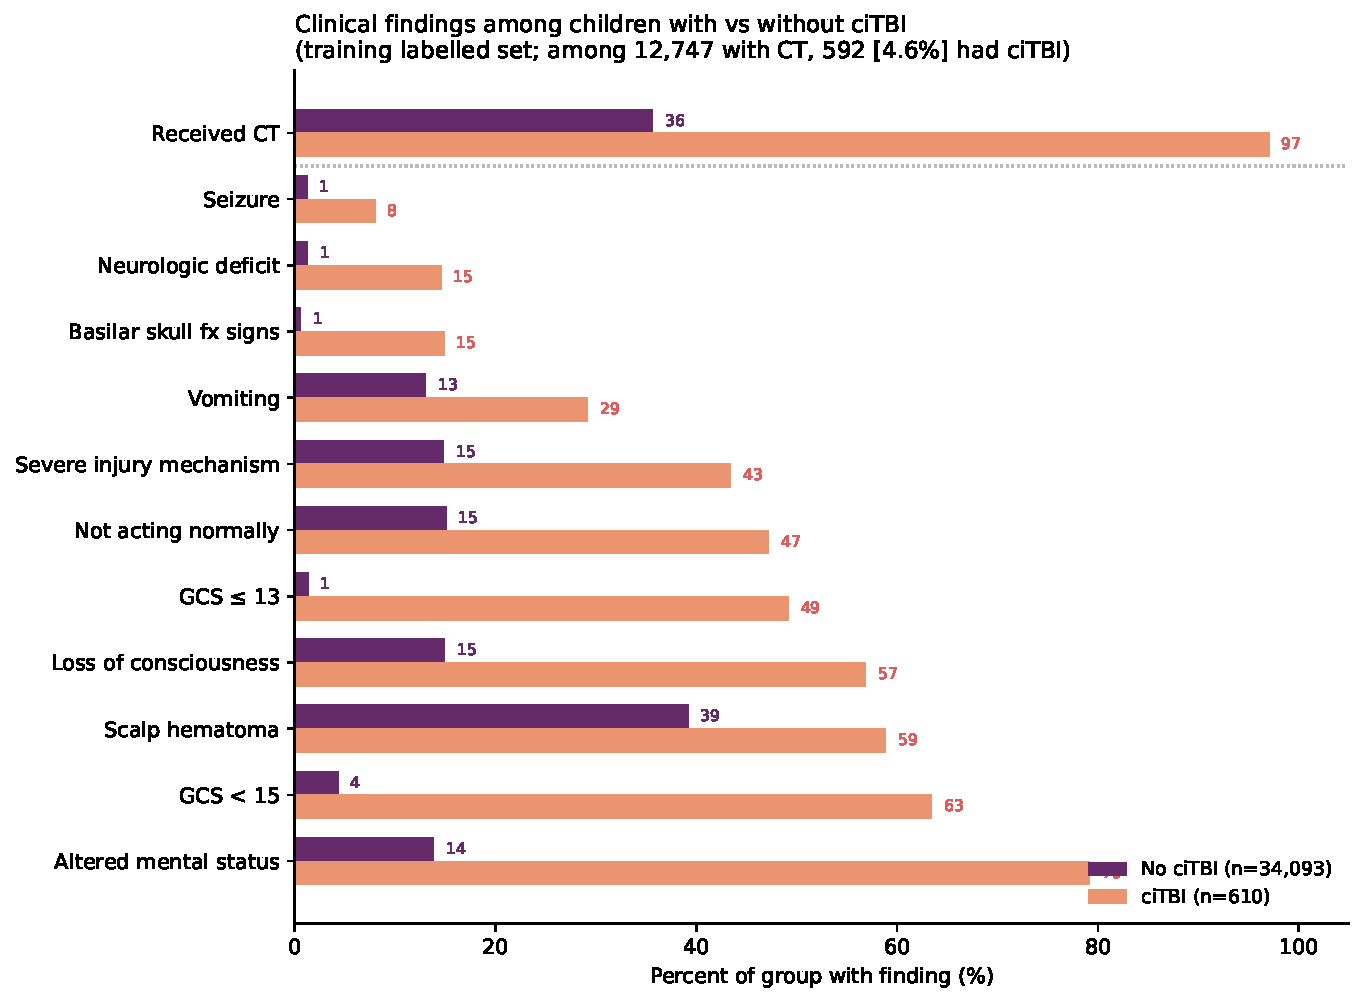
\includegraphics[width=\linewidth]{exploratory_figures/12_citbi_vs_traits.pdf}
\caption{Prevalence of selected clinical findings among children with vs without ciTBI on the training labelled set. The top row shows CT use; the title notes that only 4.6\% of children who received a CT had ciTBI.}
\label{fig:citbi-traits}
\end{figure}

\subsection{Second finding: the data is mostly populated with relevant clinical data, with low `true' missing data.}\label{second-finding}

Finding two is more of an intermediate finding, but it is notable. After cleaning up all of the duplications of children branches, etc., there is actually very limited missing data in the dataset. Figure~\ref{fig:availability} (bottom panel: true blanks only) shows that after cleaning, there are very few clinical predictors with a $>3\%$ true-missing rate; the main exceptions are \texttt{Dizzy} and \texttt{Ethnicity}. Low true missingness on AMS/GCS/LOC-type fields means a low-risk score can rely on informative clinical predictors. The top panel still shows high unavailable rates for some fields (e.g.\ amnesia, \texttt{High\_impact\_InjSev}) when 91/92 are counted with blanks, but that is mostly structural coding rather than true missingness. Given that Dizzy and Ethnicity are easy to collect, one piece of field-relevant advice from this research lab is that for future iterations, physicians and other relevant data collectors present at the hospital are encouraged to try to collect them.

\begin{figure}[H]
\centering
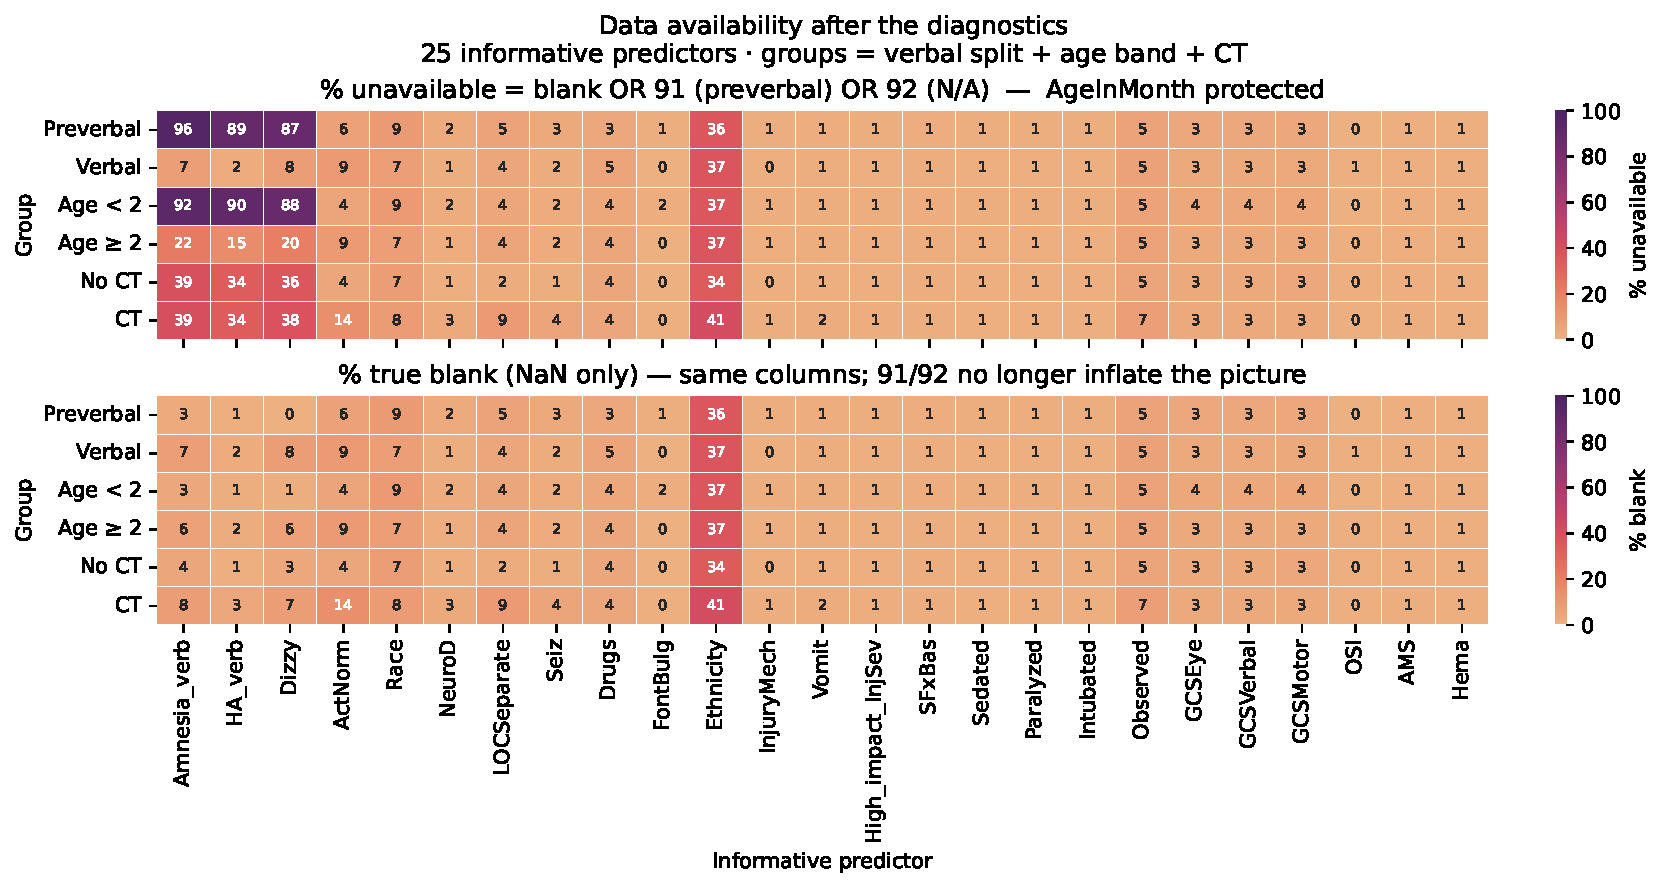
\includegraphics[width=\linewidth,height=0.48\textheight,keepaspectratio]{exploratory_figures/04_availability_after_diagnostics.pdf}
\caption{Availability of informative predictors after diagnostics, by verbal status, age band, and CT (top: blank/91/92; bottom: true blanks only).}
\label{fig:availability}
\end{figure}

\subsection{Reality Check}\label{reality-check}
I can compare this cleaned data to another source of data that discusses the same issue.
For instance, in Kuppermann's paper~\cite{kuppermann2009}, they report overall ciTBI as 0.9\%, in the slices of patients with GCS scores of 14--15.
\textbf{Assumption:} if I restrict to the same GCS 14--15 blunt-head-trauma slice that Kuppermann reports, my cleaned cohort should reproduce a similar ciTBI rate if coding and outcome definitions were not badly distorted by cleaning.
The data that I'm using also includes patients with lower GCS scores, but if I restrict my data to GCS 14--15, it matches the paper almost exactly: $n=42{,}412$, ciTBI 376 (0.89\%).
\textbf{Pass:} that agreement supports treating the cleaned frame as epidemiologically on-target for the PECARN low-risk screening setting.
What would worry me is a large mismatch (e.g.\ ciTBI rate far from $\sim$0.9\% in the GCS 14--15 slice), which would suggest outcome or GCS coding problems before any modeling.

% \begin{itemize}
% \item Do a reality check. What reality could you compare your cleaned data to?
% \item Clearly state your assumptions and explain why this reality check is useful.
% \item Does your cleaned data pass the reality check or are there issues? Discuss.
% \end{itemize}

\subsection{Stability Check}\label{stability-check}
One question is, do the high-level summary statistics from Figure~\ref{fig:citbi-traits} hold up when we perturb the data? In some sense, does the ciTBI-vs-not pattern hold in particular subpopulations?
These subpopulations are: CT vs no-CT; preverbal vs verbal; and intubated/sedated vs neither.
Verbal status is fairly stable: in Figure~\ref{fig:finding1-stability}C, the prevalence gaps for preverbal and verbal children track each other closely for most findings (with overlapping $\pm 1$ SE bars), so the ranking of mainly related signs does not depend strongly on the preverbal/verbal split; however, there is some splitting on some other traits (e.g. altered mental status and GCS).
By contrast, the no-CT and intubated/sedated cohorts are much smaller (especially no-CT ciTBI, $n_+=18$), and Panel B and D show larger shifts and wider uncertainty. Those comparisons demonstrate that there are potentially substantial differences in these subpopulations compared to the overall training set for which traits someone with a ciTBI is more likely to have.
Clinically, that means I would trust a single low-risk / skip-CT story more for preverbal vs verbal splits than for no-CT or intubated/sedated children: those groups are too thin (and possibly too different) to assume the same trait ranking or screening rule applies without more data or a group-specific rule.
We'll further explore related tradeoffs when we move on to the modeling section.

\begin{figure}[H]
\centering
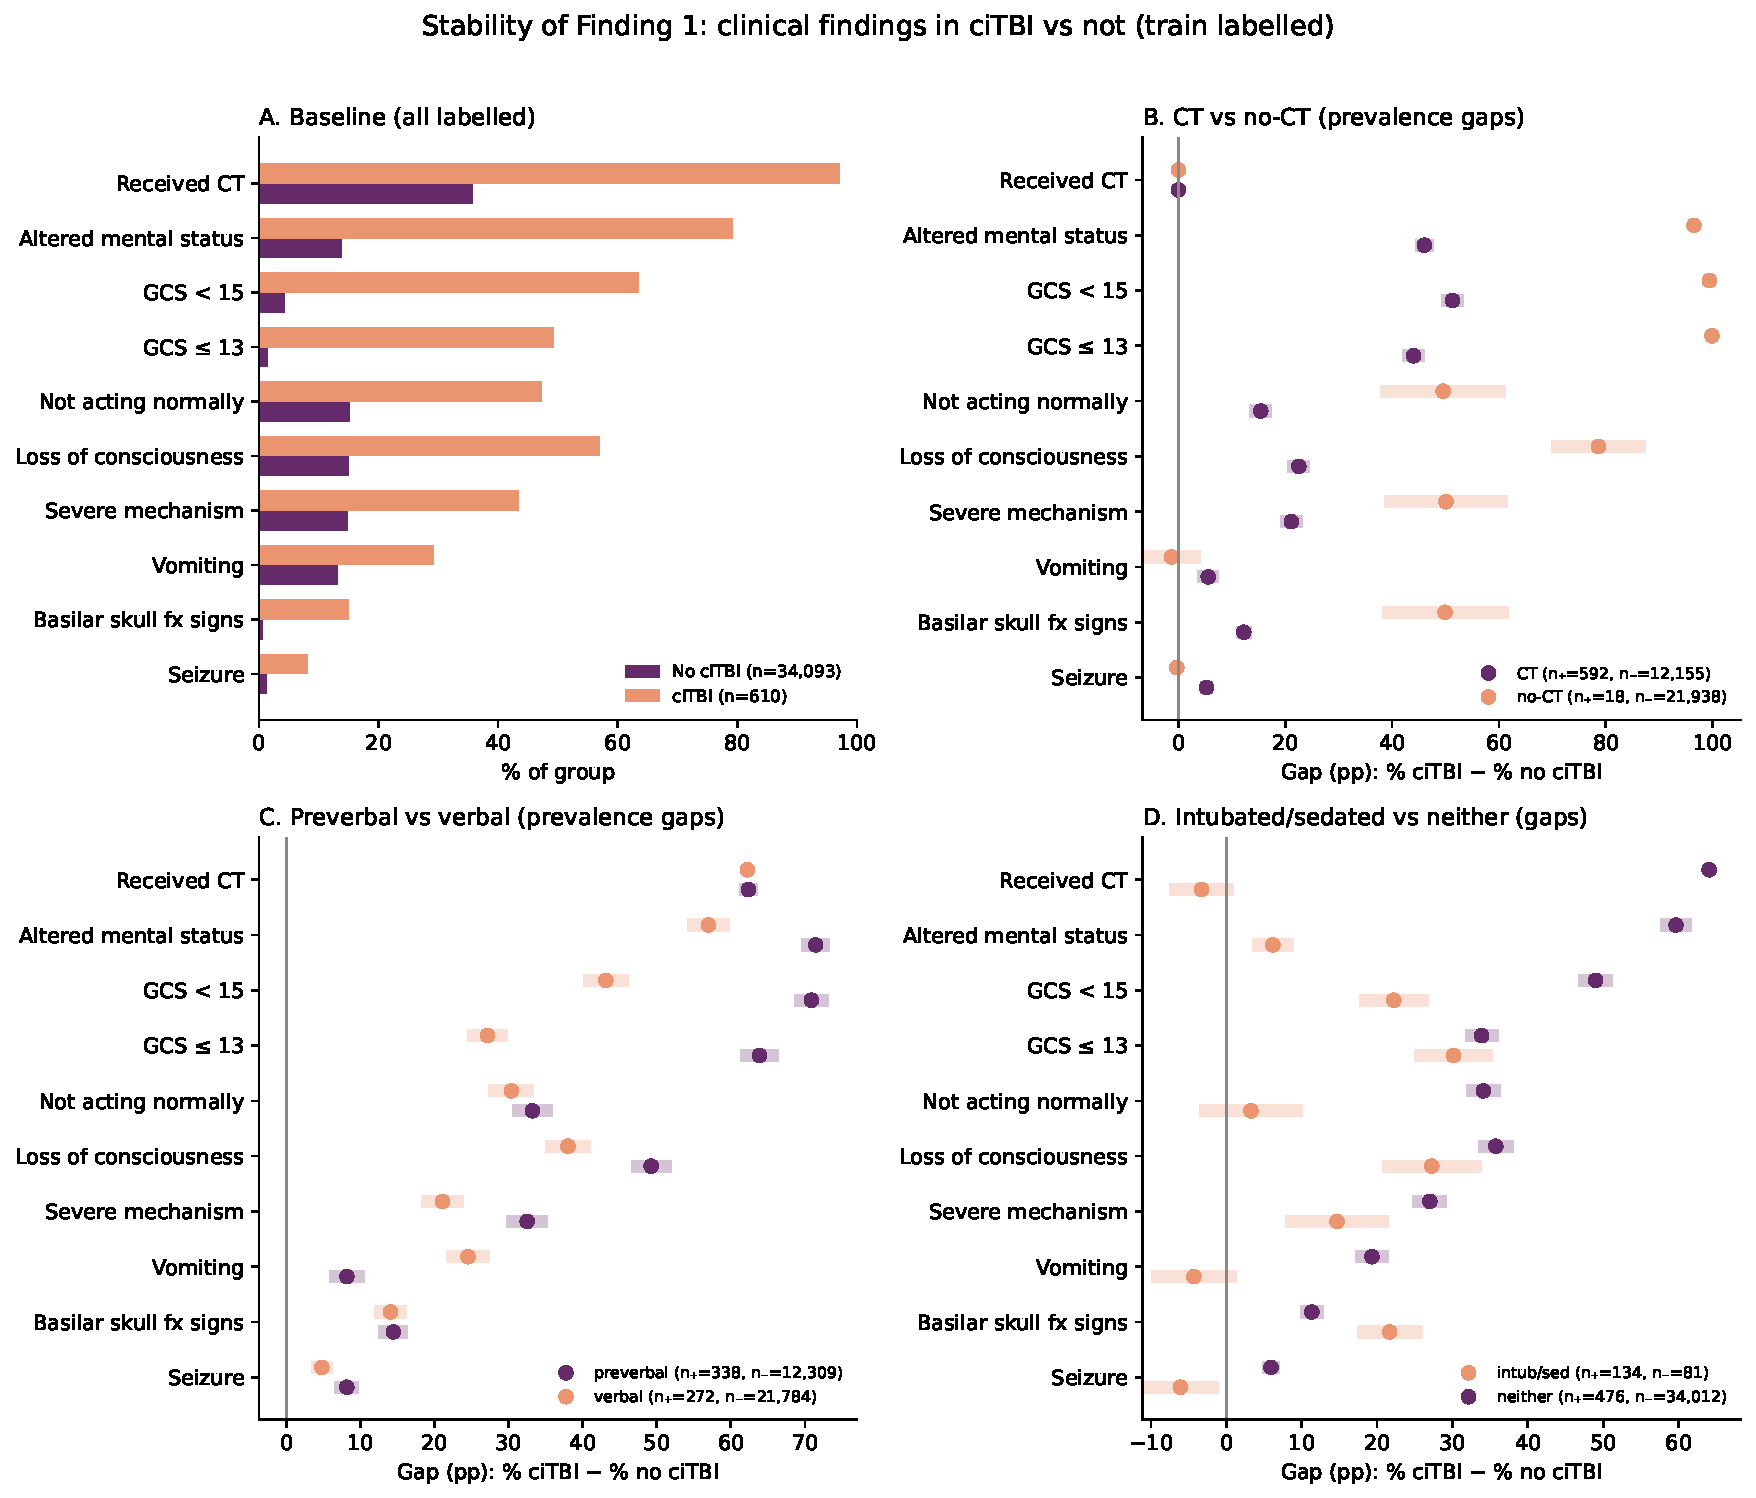
\includegraphics[width=\linewidth]{exploratory_figures/13_finding1_stability.pdf}
\caption{Stability check for Finding~1. Panel A is the baseline trait comparison on the training labelled set. Panels B--D show the same prevalence gap (\% in ciTBI minus \% in no ciTBI) within alternate cohorts: CT vs no-CT; preverbal vs verbal; and intubated/sedated vs neither. Semi-transparent bars are $\pm 1$ SE of the difference of proportions.}
\label{fig:finding1-stability}
\end{figure}

\section{Modeling}

\subsection{Implementation}
For my two models, I picked the simple logistic for the interpretability, and histgradientboosting (henceforth referred to as HGB), which is known to be better at picking up nonlinear interactions, handling 'missingness'. 
The logistic and HGB models were stratified by preverbal vs verbal status (separate fits for each cohort), in order to account for the additional verbal fields that verbal children can provide. I also report pooled (single-model) fits for comparison.
Since false negatives are more costly than false positives, I wanted to consider this when choosing models.
For the logistic model, I used many of the sklearn defaults to keep the model simple and interpretable. The penalty was L2, and I used a balanced class weight to account for the imbalanced nature of the data.
For HGB, I also had many of the preset hyperparameters. Given the scarcity of the ciTBI events, I did not want to tune hyperparameters and risk overfitting.
Table~\ref{tab:hyperparameters} lists the settings used for both models; none were tuned on the holdout.


\begin{table}[H]
    \centering
    \caption{Hyperparameters for the logistic and HistGradientBoosting models (sklearn). Shared settings appear in both columns; NA means the setting does not apply.}
    \label{tab:hyperparameters}
    \begin{tabular}{lll}
    \hline
    Hyperparameter & Logistic & HGB \\
    \hline
    \texttt{penalty} & L2 & NA \\
    \texttt{C} & 1.0 (default) & NA \\
    \texttt{solver} & \texttt{lbfgs} (default) & NA \\
    \texttt{max\_iter} & 2000 & 300 \\
    \texttt{max\_depth} & NA & 6 \\
    \texttt{learning\_rate} & NA & 0.08 \\
    \texttt{min\_samples\_leaf} & NA & 40 \\
    \texttt{l2\_regularization} & NA & 0.1 \\
    \texttt{early\_stopping} & NA & True \\
    \texttt{validation\_fraction} & NA & 0.1 \\
    \texttt{n\_iter\_no\_change} & NA & 20 \\
    \texttt{class\_weight} & \texttt{balanced} & \texttt{balanced} \\
    \texttt{random\_state} & 215 & 215 \\
    \hline
    \end{tabular}
\end{table}

% \begin{itemize}
%     \item Since false negatives are more costly than false positives, I wanted to consider this when choosing models.
%     \item Discuss any design choices that were made in the modeling stage.
%     \begin{itemize}
%         \item Which algorithms did you use?
%         \item How did you determine hyperparameters? 
%     \end{itemize}
%     \item This should not drone on for too long, but give enough information that your implementation can be replicated by a reader.
% \end{itemize}

\begin{figure}[H]
\centering
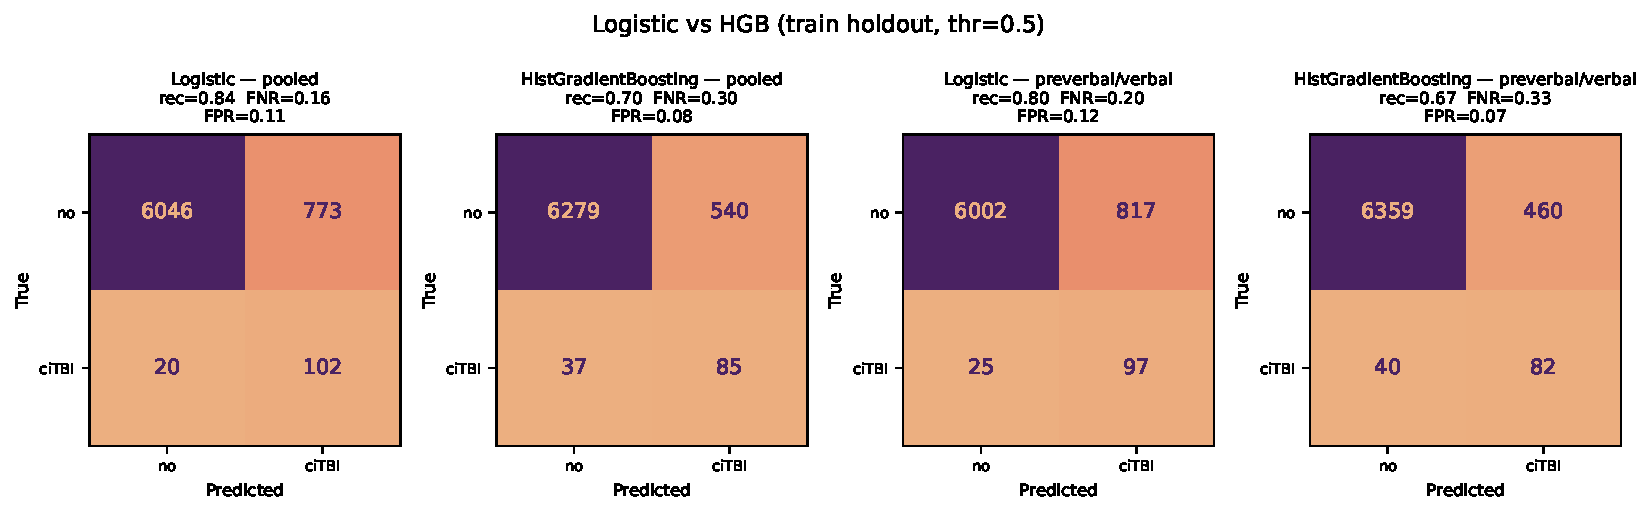
\includegraphics[width=\linewidth]{exploratory_figures/09_logistic_vs_hgb_confusion.pdf}
\caption{Train-holdout confusion matrices for pooled vs preverbal/verbal logistic and HGB (default threshold $0.5$).}
\label{fig:logistic-vs-hgb}
\end{figure}

\subsection{Stability}
In order to check the stability of the models, I applied two strategies: 1) ridge classifier, and 2) 5-fold cross validation. Both use the same preverbal/verbal stratification as the main logistic fits. The results of the stability check of the models can be found in Figure~\ref{fig:pcs-perturbation}.

\begin{figure}[H]
\centering
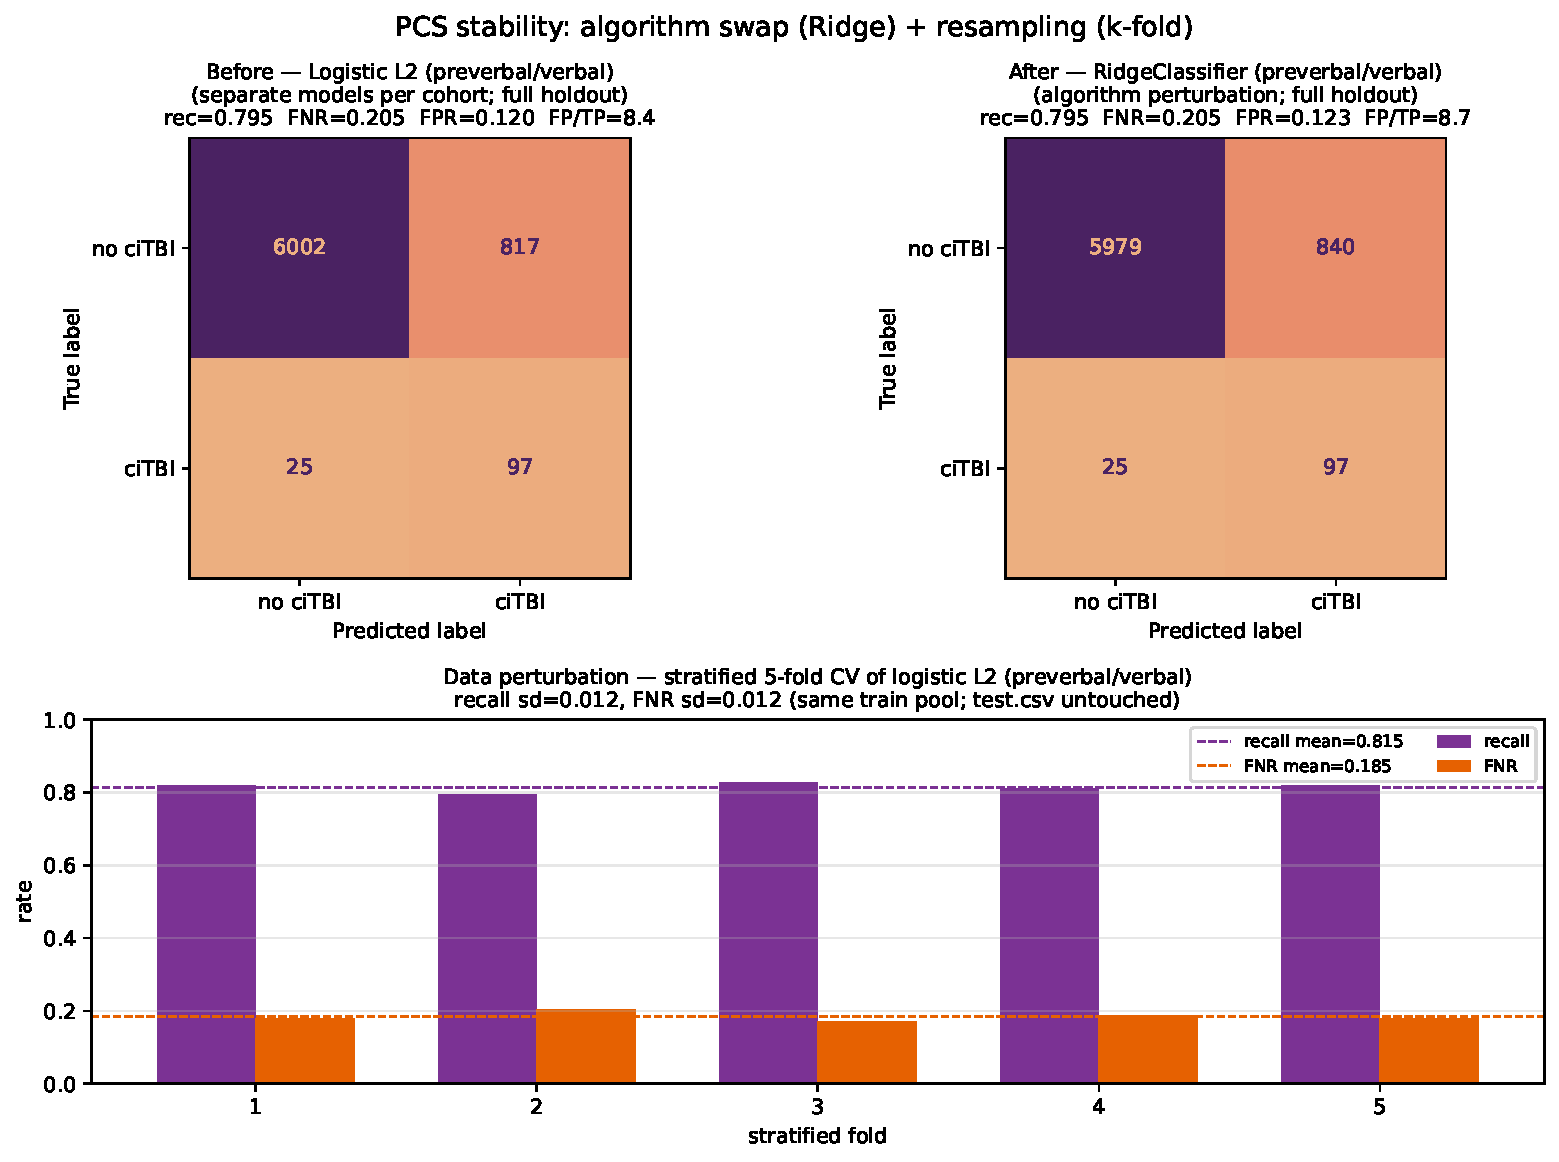
\includegraphics[width=\linewidth]{exploratory_figures/10_pcs_perturbation_stability.pdf}
\caption{One perturbation we did is to try a RidgeClassifier in place of logistic L2, both fit separately on preverbal and verbal cohorts. As you can see, the resulting confusion matrix is very similar to the one from the simple Logistic L2 (same holdout FNR $=0.205$ and recall $=0.795$; prediction agreement $0.967$). For a data perturbation, I also did a 5-fold cross validation of the same preverbal/verbal logistic. As you can see, the mean False Negative Rate (FNR) is $0.185$ over the folds, while the mean recall is $0.815$, with relatively low variation (sd $\approx 0.012$). Compare this to the original L2 on the fixed holdout, which has FNR $=0.205$ and a recall of $0.795$.}
\label{fig:pcs-perturbation}
\end{figure}

\subsection{Discussion}

I chose the logistic L2 model because it is a simple model that is easy to interpret, and well-known for being good at handling imbalanced data.
I also chose HGB because it is known to be better at picking up nonlinear interactions, and handling 'missingness'.
Figure~\ref{fig:logistic-interp} sketches how the logistic model maps clinical predictors to $P(\mathrm{ciTBI})$ and shows L2-penalized odds ratios for selected exam findings (not the PECARN rule itself).

\begin{figure}[H]
\centering
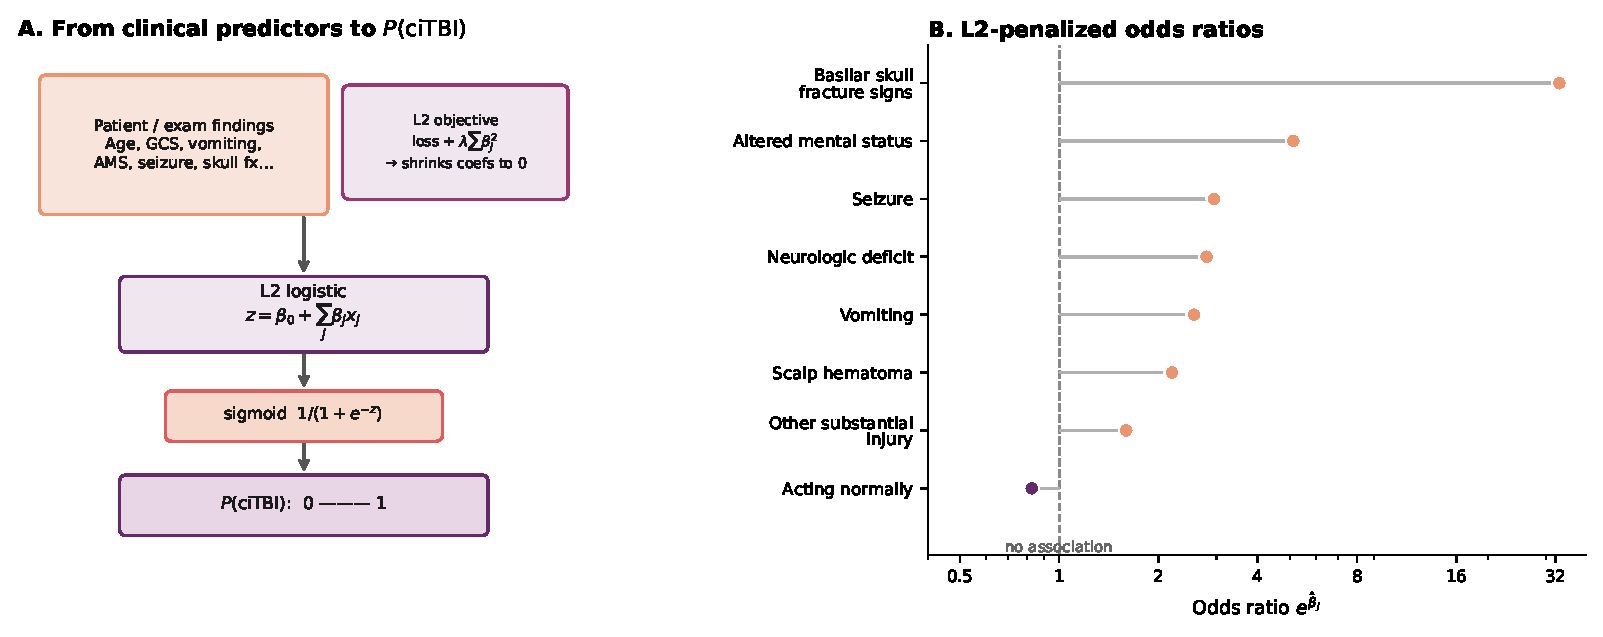
\includegraphics[width=\linewidth]{exploratory_figures/11_logistic_interpretation.pdf}
\caption{Interpretation schematic for the balanced L2 logistic model. Panel A: clinical predictors are scored through a linear log-odds, using a sigmoid to calculate the probability of ciTBI from the input data. Panel B: selected coefficients and how they influence the odds of ciTBI. For instance, AMS and skull-fracture signs push risk up; acting normally pushes it down a little relative to baseline.}
\label{fig:logistic-interp}
\end{figure}

I also ran two different runs of both the logistic and HGB models: one for the pooled data (mixing preverbal and verbal children), and one for the verbal-stratified data (separating children who are preverbal from those who are verbal).
I chose to do this because I assumed that given that the verbal children are able to provide more information, the models might be able to pick up patterns for the verbal children that differ from the preverbal children, due to lack of information.
My choice was also partially informed from Figure~\ref{fig:finding1-stability}, where I saw there was a small difference in some metrics that are easier to measure in verbal children (e.g. altered mental status).
Overall, on the test set the false positive rate for HGB is lower (lower by about 30--40\% compared to the FPR for logistic), but the false negative rate is almost twice as high. Given that it is so much more costly to miss a ciTBI, I would preferably use the simpler logistic model over the HGB.

Table~\ref{tab:final-test} reports the one-time evaluation on the frozen test set ($n=8{,}676$, 153 ciTBI), after fitting on the full training modelling frame. Development figures above used a train holdout only; these numbers were not used for model selection.

\begin{table}[H]
    \centering
    \caption{Final frozen-test performance (threshold $0.5$). TP/FP/FN/TN are counts; FNR and FPR are rates.}
    \label{tab:final-test}
    \begin{tabular}{lrrrrrr}
    \hline
    Model & TP & FP & FN & TN & FNR & FPR \\
    \hline
    Logistic pooled & 136 & 853 & 17 & 7{,}670 & 0.111 & 0.100 \\
    Logistic preverbal/verbal & 137 & 925 & 16 & 7{,}598 & 0.105 & 0.109 \\
    HGB pooled & 127 & 666 & 26 & 7{,}857 & 0.170 & 0.078 \\
    HGB preverbal/verbal & 124 & 562 & 29 & 7{,}961 & 0.190 & 0.066 \\
    \hline
    \end{tabular}
\end{table}

Through using this simple logistic preverbal/verbal screen, there would just be 16 FNs per 153 ciTBI patients (FNR $=0.105$) vs 925 FP (extra ``would-scan'' among non-ciTBI).
So among kids without ciTBI, about 1 in 9 get flagged; given that most patients do not have ciTBI, that is a large absolute number.
I prefer this logistic screen over HGB because missing ciTBI is costlier than extra CTs, even though HGB has fewer false positives.
However, this model can still be improved on to further lower the FNR; which, if it gets low enough, and implemented at scale, would reduce unnecessary cancer and leukemia chance in young patients~\cite{pearce2012,miglioretti2013}.
Unlike the PECARN clinical decision rules~\cite{kuppermann2009}, which are age-specific checklists with validation sensitivity 96.8--100\% (FNR $\approx$ 0--3\%) but specificity only about 54--60\% (FPR $\approx$ 40--46\%), my logistic model is a learned score at a fixed $0.5$ threshold (test specificity $\approx$ 89\%, FPR $\approx$ 0.11, but much higher FNR) and was not evaluated as Kuppermann's rule on the same test frame, so these results should not be read as clinical readiness relative to PECARN.

% \begin{itemize}
%     \item why did you choose to try these two models
%     \item Is your model a simple interpretable form?
%     \item If not, how do you recommend interpreting how it
% obtains the predictions it does?
% \end{itemize}

% If possible, include a figure or schematic that explains how one of your models works.

\section{Conclusion}\label{conclusion}
Overall, the plan and strategy I used for this work is in line with the Data Science Life Cycle with the PCS lens.
In the PCS framing, the lab parts map onto three realms as follows.

\textbf{Data / reality.}
How the table relates (or fails to relate) to the clinical world.
There was some missing data (e.g.\ ethnicity) that could have been useful.
Also, it is important to keep in mind before we begin analyzing the data that in practice it may simply not be possible to implement the suggestions or strategies we have here, as doctors may face legal limitations, concerns from patients, and other constraints.
In addition, this is when researchers need to look at the limitations of this data and foresee potential issues with the cleaning process and how we apply the models.
There were some limitations with the data, and how I expect it generalizes to reality.
The data size restricted me for some subexperiments I wanted to run. For some of the ways it made sense to ``split'' the data (aside from the preverbal and verbal split I did for the models, given that the preverbal children were not able to provide as much information), there were not enough patients for different ``cohorts'' to be run through the model. For instance, the intubated/sedated vs neither split had some differences in the ciTBI and no ciTBI feature proportions that we graphed in Figure~\ref{fig:finding1-stability}, but the dataset size for intubated/sedated was less than 1\% of the total dataset (215 of $34{,}703$ training labelled patients, about $0.6\%$).
I do not think there is a one-to-one correspondence of the data and reality. Firstly, the data was collected by physicians who were part of the 25 participating locations for PECARN.
There are some limitations for how effectively the visualizations can be used to represent reality: for instance, there are many top 'input' values that influence the model prediction, but including all of them in Figure~\ref{fig:logistic-interp} would have made it difficult to read.
However, data visualization was incredibly useful for this lab, as it allows us to quickly see patterns. This was especially effective in Figure~\ref{fig:finding1-stability}, where I had four subpanels showing the difference between prevalence of different input values (like low GCS) for those with ciTBI, and those without, much more effectively than showing a list or a table.

\textbf{Algorithms / models.}
How we turned the cleaned data into predictions with models, and how interpretable and stable our models are.
Using the PCS framework, I checked for stability using both a Ridge swap and 5-fold CV, to ensure stability of predictions under algorithm and sample perturbation.
In addition, under the guidance of the PCS framework, decisions like choosing logistic over HGB were clearly explained and documented (e.g.\ due to the researcher making a decision that false negatives are more costly than false positives, and thus ruling in favour of the logistic model).

\textbf{Future data / prediction.}
What happens when we apply the fitted story to new patients, or patients outside this cohort?
I tried to simulate this with the frozen 80/20 split, where cleaning was only decided from the training set, and later applied to the testing set after I had already trained and chosen my models.
This simulates ``future'' patients by ensuring that their data is not being used to build the pipeline.
However, some limitations I foresee are that there might be changes in site or default practices, and thus future data we collect might not look like that from the PECARN dataset; we may also have additional input variables that can be even more informative.
Other systems and hospitals may have different data collection practices, and might not collect data in the same manner, which can influence results if we attempt to apply the models to that data.

Overall, the PECARN data is large, detailed, and contains a lot of information about each patient that can be used to make an effective model that can help reduce overscreening of children that are at low risk of having a clinically important TBI.
This was demonstrated through my preliminary explorations of the data, where even simple models (like the Logistic L2) were able to pick up some patterns from clinical data to identify children that are at low risk of a ciTBI with a relatively small false negative rate on the test dataset.


% Provide an overall assessment and discussion of your work as an example of a Data Science Life Cycle with
% the PCS lens.
% Address the three realms: data / reality, algorithms / models, and future data / reality.
% Where do the parts of the lab fit into those three realms?
% Did the data size restrict you in any way? Discuss some challenges that you faced as a result of the
% data size.
% Do you think there is a one-to-one correspondence of the data and reality?
% What about reality and data visualization?
% You should make attempts to connect your findings/analysis back to the domain problem in every
% section of this report, but here in the conclusion, you can reiterate your main points and provide
% overarching remarks on the PECARN data as it relates to the domain problem

\section{Academic honesty statement}\label{academic-honesty-statement}

Dear reader, the work in this report is done by me, and all sources I used were properly cited.  Academic research honesty is important for progress (otherwise we run into situations like where the guy from Berkeley pretended to have made+detected heavier atoms and then he, in fact, had not and this messed up our understanding of chem for a while).

\section{Collaborators}\label{collaborators}

I had no collaborators for this lab. I used various LLM models through Cursor in order to draft various functions used in the code, in a manner that I discussed and got approval from Anqi beforehand.

\section{Bibliography}\label{bibliography}

% thebibliography would otherwise print a "References" heading
\renewcommand{\refname}{}
\makeatletter
\renewenvironment{thebibliography}[1]
     {\list{\@biblabel{\@arabic\c@enumiv}}%
           {\settowidth\labelwidth{\@biblabel{#1}}%
            \leftmargin\labelwidth
            \advance\leftmargin\labelsep
            \@openbib@code
            \usecounter{enumiv}%
            \let\p@enumiv\@empty
            \renewcommand\theenumiv{\@arabic\c@enumiv}}%
      \sloppy
      \clubpenalty4000
      \@clubpenalty \clubpenalty
      \widowpenalty4000%
      \sfcode`\.\@m}
     {\def\@noitemerr
       {\@latex@warning{Empty `thebibliography' environment}}%
      \endlist}
\makeatother

\begin{thebibliography}{9}

\bibitem{kuppermann2009}
N. Kuppermann, J. F. Holmes, P. S. Dayan, et al.,
``Identification of children at very low risk of clinically-important brain injuries after head trauma: a prospective cohort study,''
\textit{The Lancet},
vol. 374, no. 9696, pp. 1160--1170, 2009.
doi: 10.1016/S0140-6736(09)61558-0.

\bibitem{miglioretti2013}
D. L. Miglioretti, E. Johnson, A. Williams, et al.,
``The use of computed tomography in pediatrics and the associated radiation exposure and estimated cancer risk,''
\textit{JAMA Pediatrics},
vol. 167, no. 8, pp. 700--707, 2013.
doi: 10.1001/jamapediatrics.2013.311.

\bibitem{pearce2012}
M. S. Pearce, J. A. Salotti, M. P. Little, et al.,
``Radiation exposure from CT scans in childhood and subsequent risk of leukaemia and brain tumours: a retrospective cohort study,''
\textit{The Lancet},
vol. 380, no. 9840, pp. 499--505, 2012.
doi: 10.1016/S0140-6736(12)60815-0.

\end{thebibliography}

\end{document}